\documentclass{article}



% Language setting

% Replace `english' with e.g. `spanish' to change the document language

\usepackage[english]{babel}



% Set page size and margins

% Replace `letterpaper' with `a4paper' for UK/EU standard size

\usepackage[letterpaper,top=2cm,bottom=2cm,left=3cm,right=3cm,marginparwidth=1.75cm]{geometry}



% Useful packages

\usepackage{amsmath}

\usepackage{amssymb}

\usepackage{graphicx}

\usepackage[colorlinks=true, allcolors=black]{hyperref}

\usepackage{titlesec}
\usepackage{xparse}



\NewDocumentCommand{\qcq}{m o o m}{%
	\ensuremath{\forall #1 \IfValueT{#2}{, #2} \IfValueT{#3}{, #3}  \in  \mathbb{#4}}%
}
\NewDocumentCommand{\ext}{m o o m}{%
	\ensuremath{\exists #1 \IfValueT{#2}{, #2} \IfValueT{#3}{, #3}  \in  \mathbb{#4}}%
}



\title{\textbf{Rappels et compléments de calcul}}

\author{\textbf{Yassin Akkab}}



\newcommand{\R}{\mathbb{R}}
\newcommand{\N}{\mathbb{N}}
\newcommand{\Z}{\mathbb{Z}}
\newcommand{\C}{\mathbb{C}}
\newcommand{\Q}{\mathbb{Q}}
\newcommand{\D}{\mathbb{D}}





\graphicspath{ {./Screenshots/} }




\begin{document}
	
	\maketitle
	
	
	
	\tableofcontents
	
	\newpage
	
	\section{Les ensembles de nombres usuels}
	\subsection{Définition}
	On définit les ensembles de nombres suivants : 
	\begin{enumerate}
		\item $ \mathbb{N} = \{0, 1, 2, 3, \ldots\} $ l'ensemble des entiers naturels ;
		\item $ \mathbb{Z}= \N \cup -\N  = \{\dots,-2,-1,0,1,2,\dots \} $ l'ensemble des entiers relatifs ;
		\item $\Q = \{\frac{p}{q} | p,q \in \Z, q \neq 0\} $
		\item $\R$ l'ensemble des abscisses d'une droite graduée, l'ensemble des réels;
		\item $\C$ l'ensemble nombres de la forme $a+ib$ ou a,b $\in$ $\R$ et $i^2 = -1$, l'ensemble des complexes.
		
	\end{enumerate}

	Et on note $\N^*, \Q^*,\R^*, \C^*$ les memes ensembles privés de 0.
	
	L'ensemble $\R \backslash \Q$ est appelé l'ensemble des irrationnels.
	
	On considère parfois aussi l'ensemble $\D$ des nombres décimaux : $\D$ = \{$\frac{n}{10^m}|n,m \in \Z$ \}

	\begin{figure}[h]
		\centering
		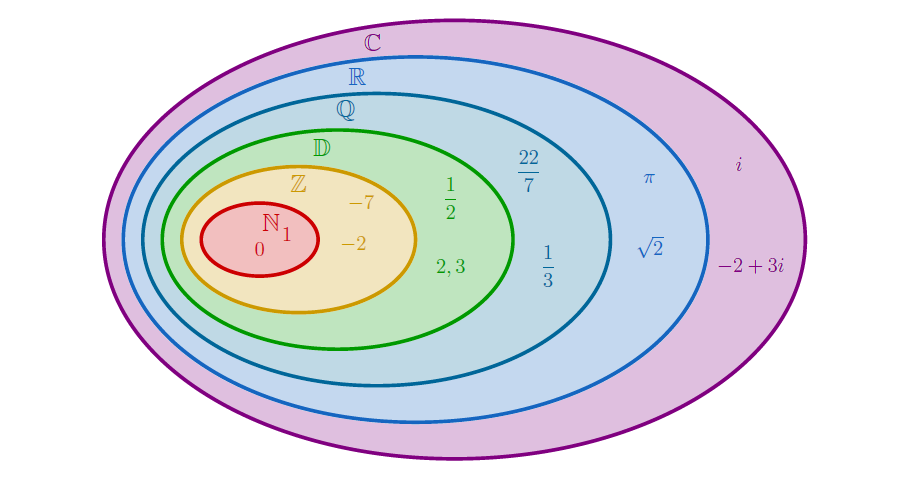
\includegraphics[width=0.7\textwidth]{image1.png}
	\end{figure}
	
	\section{Intervalles et inégalités dans $\R$}
	
	\subsection{Définition}
	Si $a, b \in \mathbb{R}$, on définit le segment $[a; b]$ comme :
	\[ [a; b] = \{x \in \mathbb{R} \,|\, a \leq x \leq b\}. \]
	On dit qu'un ensemble non vide $I$ de $\mathbb{R}$ est un intervalle s'il vérifie que :
	\[ \forall a, b \in I, [a; b] \subset I. \]
	
	\subsection{Remarque }
	Cela revient à dire qu'un intervalle contient tous les réels entre ses éléments.
	
	\subsection{Exemples }
	\begin{enumerate}
		\item Si $a \in \mathbb{R}$, l'ensemble $I = \{a\}$ est un intervalle : il est non vide, et si $a, b \in I$, et $x \in [a; b]$, alors $a = b$ et ainsi : $a \leq x \leq a$, donc $x = a$ appartient bien à $I$.
		\item Tout segment est un intervalle : si $I = [a; b]$ et $a', b' \in I$, alors :
		\[ x \in [a'; b'] \Rightarrow a' \leq x \leq b' \Rightarrow a \leq a' \leq x \leq b' \leq b \Rightarrow a \leq x \leq b \Rightarrow x \in I. \]
		\item $\mathbb{N}$ n'est pas un intervalle car : $0 \in \mathbb{N}$ et $1 \in \mathbb{N}$, mais $\frac{1}{2} \in [0; 1]$ n'est pas dans $\mathbb{N}$, donc on n'a pas l'inclusion $[0; 1] \subset \mathbb{N}$.
	\end{enumerate}
	
	\subsection{Proposition}
	Tout intervalle non vide de $\mathbb{R}$ est d'une (et une seule) des formes suivantes, où $a$ et $b$ désignent des réels tels que $a < b$ :
	\begin{enumerate}
		\item $\{a\}$ ;
		\item $[a; b] = \{x \in \mathbb{R} \,|\, a \leq x \leq b\}$ ;
		\item $[a; b[ = \{x \in \mathbb{R} \,|\, a \leq x < b\}$ ;
		\item $]a; b] = \{x \in \mathbb{R} \,|\, a < x \leq b\}$ ;
		\item $]a; b[ = \{x \in \mathbb{R} \,|\, a < x < b\}$ ;
		\item $[a;+\infty[ = \{x \in \mathbb{R} \,|\, a \leq x\}$ ;
		\item $]a;+\infty[ = \{x \in \mathbb{R} \,|\, a < x\}$ ;
		\item $]-\infty; b] = \{x \in \mathbb{R} \,|\, x \leq b\}$ ;
		\item $]-\infty; b[ = \{x \in \mathbb{R} \,|\, x < b\}$ ;
		\item $\mathbb{R}$.
	\end{enumerate}
	
	\subsection{Définition }
	Les intervalles précédents définis par des inégalités strictes sont appelés des intervalles ouverts.
	Plus généralement, si $I$ est un intervalle, on appelle intérieur de $I$, noté $\stackrel{\circ}{I}$, l'intervalle $I$ privé de ses bornes.
	
	\subsection{Remarque }
	Prendre l'intérieur, c'est "ouvrir" l'intervalle : $\stackrel{\circ}{I}$ est le plus grand intervalle ouvert inclus dans $I$.
	
	\section{ Racines et puissances}
	
	\subsection{Définition }
	Si $x \geq 0$, on appelle sa racine carrée, notée $\sqrt{x}$, comme l'unique réel positif ou nul dont le carré vaut $x$.
	
	\subsection{Remarque }
	Comme $x^2 = (-x)^2$, alors
	\[ \sqrt{x^2} =
	\begin{cases}
		x & \text{si } x \geq 0, \\
		-x & \text{si } x \leq 0.
	\end{cases}
	\]
	
	\subsection{Proposition }
	Soient $x$ et $y$ positifs. Alors :
	\[ \sqrt{xy} = \sqrt{x} \sqrt{y} \]
	et
	\[ \sqrt{xy} = \sqrt{x} \sqrt{y} \text{ (si } y \neq 0 \text{).}\]
	
	\textbf{Démonstration.} Par définition, on a $\sqrt{x}$ et $\sqrt{y}$ sont positifs, donc leur produit aussi. Et :
	\[
	\left(\sqrt{x} \sqrt{y}\right)^2 = (\sqrt{x})^2 (\sqrt{y})^2 = xy
	\]
	d'où la première égalité. On procède de même pour le quotient.
	
	\subsection{Remarques }
	1. On utilise les carrés parfaits pour simplifier les racines : $1, 4, 9, 16, 25, 36, \ldots, 289, 324, 361, \ldots$.
	2. On évite de garder des racines au dénominateur dans un quotient. On simplifie une fraction en multipliant par $\sqrt{a}$, $\sqrt{a} - \sqrt{b}$ ou $\sqrt{a} + \sqrt{b}$ pour les faire disparaître.
	
	\subsection{Exemples}
	\begin{enumerate}
		\item $\sqrt{180} = \sqrt{36 \times 5}  = 6\sqrt{5}$.
		\item $\sqrt{\frac{3}{5}} = \frac{\sqrt{15}}{5} $.
		\item $\frac{1}{\sqrt{11} - \sqrt{3}} =\frac{\sqrt{11} + \sqrt{3}}{8}  $.
	\end{enumerate}

	
	\subsection{Définition }
	Si $x \in \mathbb{R}$ et $n \in \mathbb{N}$, on note :
	\[ x^n =
	\begin{cases}
		1 & \text{si } n = 0, \\
	 x^n = \underbrace{x \cdot x \cdot \ldots \cdot x}_{\text{n fois}}
	
	\end{cases}
	\]
	Si $x \neq 0$ et $n \in \mathbb{Z}^{-}$, on note :
	\[ x^n =
	\left(\frac{1}{x}\right)^{-n} = \frac{1}{\underbrace{x \cdot x \cdot \ldots \cdot x}_{\text{n fois}} 
	}.
	\]
	
	\subsection{Proposition }
	Si $x, y \in \mathbb{R}$ et $n, m \in \mathbb{N}$ :
	\[ x^{m + n} = x^m \cdot x^n, \]
	\[ x^{mn} = (x^m)^n = (x^n)^m, \]
	\[ (xy)^n = x^n y^n, \]
	et ces formules restent valables pour $n, m \in \mathbb{Z}$ si $x, y \neq 0$.
	\section{La valeur absolue}
	
	\subsection{Définition }
	Si $x \in \mathbb{R}$, on appelle valeur absolue de $x$, notée $|x|$, le réel :
	\[
	|x| =
	\begin{cases}
		x & \text{si } x \geq 0 \\
		-x & \text{si } x < 0
	\end{cases}
	\]
	
	\subsection{Remarques }
	\begin{enumerate}
		\item Une valeur absolue est toujours positive ou nulle.
		\item Si $x \in \mathbb{R}$ : $-|x| \leq x \leq |x|$, et l'une des deux inégalités est une égalité.
	\end{enumerate}
	
	\subsection{Proposition }
	Si $x, y \in \mathbb{R}$ :
	\begin{enumerate}
		\item $|x| = \sqrt{x^2}$
		\item $|x| = 0 \Leftrightarrow x = 0$
		\item $|xy| = |x| \cdot |y|$ et $\frac{x}{y} = \frac{|x|}{|y|}$ (pour $y \neq 0$)
		\item $|x| = |y| \Leftrightarrow x^2 = y^2 \Leftrightarrow (x = y$ ou $x = -y)$
		\item $|x| \leq y \Leftrightarrow -y \leq x \leq y$ et $|x| \geq y \Leftrightarrow x \geq y$ ou $x \leq -y$
	\end{enumerate}
	
	\subsection{Démonstration}
	\begin{enumerate}
		\item Déjà vu avec les racines.
		\item Clair.
		\item Découle du 1.
		\item Par le 1., on a déjà : $|x| = |y| \Leftrightarrow \sqrt{x^2} = \sqrt{y^2}$ :
		- Si $\sqrt{x^2} = \sqrt{y^2}$ : en élevant au carré, on a : $x^2 = y^2$.
		- Si $x^2 = y^2$ : en prenant la racine carrée, on a $\sqrt{x^2} = \sqrt{y^2}$, ce qui donne déjà que $|x| = |y| \Leftrightarrow x^2 = y^2$. Et on utilise enfin que :
		$x^2 = y^2 \Leftrightarrow x^2 - y^2 = 0 \Leftrightarrow (x - y)(x + y) = 0 \Leftrightarrow
		\begin{cases}
			x = y \\
			\text{ou} \\
			x = -y
		\end{cases}$
		\item On procède par disjonction de cas : \newline
		- Si $x \geq 0$ : alors $|x| = x$ et donc : 
		$|x| \leq y \Leftrightarrow 0 \leq x \leq y \Leftrightarrow -y \leq 0 \leq x \leq y \Leftrightarrow -y \leq x \leq y$. \newline
		- Si $x \leq 0$ : alors $|x| = -x$ et donc :
		$|x| \leq y \Leftrightarrow 0 \leq -x \leq y \Leftrightarrow -y \leq -x \leq y$
	\end{enumerate}
		\subsection{Remarques }
		\begin{enumerate}
			\item Si $y < 0$, alors les équivalences sont triviales (dans le sens où elles sont non seulement évidentes, mais qu'en plus elles n'apportent rien comme information) :
			- L'inégalité $|x| \leq y$ sera toujours fausse, de même que l'inégalité $-y \leq x \leq y$ (car elle impliquerait que $-y \leq y$, ce qui est évidemment faux).
			- L'inégalité $|x| \geq y$ sera toujours vraie, comme le fait que $x \geq y$ ou que $x \leq -y$. On a en effet : $x \geq y \Leftrightarrow x \in [y;+\infty[$ et $x \leq -y \Leftrightarrow x \in] -\infty; -y]$ et l'union de ces deux intervalles forme bien toute la droite des réels.
			\item Si $y \geq 0$, on a même : $|x| \leq y \Leftrightarrow x^2 \leq y^2$ et $|x| \leq y \Leftrightarrow x^2 \leq y^2$.
		\end{enumerate}
		
		\subsection{Corollaire}
		Si $a, b \in \mathbb{R}$ avec $b > 0$, l'ensemble des réels $x$ tels que $|x - a| \leq b$ est le segment $[a - b; a + b]$.
		
		\subsection{Définition}
		Si $x, y \in \mathbb{R}$, la quantité $|x - y|$ est appelée distance entre $x$ et $y$.
		
		\subsection{Remarque }
		L'intervalle $[a - b; a + b]$ correspond à l'ensemble des réels à distance au plus $b$ de $a$.
		
		\subsection{Théorème (Inégalité triangulaire)}
		Si $x, y \in \mathbb{R}$, alors :
		\begin{enumerate}
			\item $|x + y| \leq |x| + |y|$
			\item $||x| - |y|| \leq |x - y|$
		\end{enumerate}
		De plus, il y a égalité dans les deux cas si, et seulement si, $x$ et $y$ sont de même signe.
		
		Démonstration. 
		\begin{enumerate}
			\item On utilise que $-|x| \leq x \leq |x|$ et $-|y| \leq y \leq |y|$. \\
			 Donc : $- (|x| + |y|) \leq x + y \leq |x| + |y|$. \\
			  D'où : $|x + y| \leq |x| + |y|$.
			\item On utilise l'inégalité précédente : \\ $|x| = |(x - y) + y| \leq |x - y| + |y|$,\\ donc $|x| - |y| \leq |x - y|$. \\ En échangeant les rôles de $x$ et $y$, on trouve : \\ $|y| - |x| \leq |y - x| = |x - y|$. \\ Donc : $-|x - y| \leq |x| - |y| \leq |x - y|$. Et ainsi : $||x| - |y|| \leq |x + y|$. \\ Pour les égalités, on a : $|x + y| = |x| + |y| \Leftrightarrow (x + y)^2 = (|x| + |y|)^2 \Leftrightarrow xy = |x| \cdot |y| = |xy| \Leftrightarrow xy \geq 0$. $||x| - |y|| = |x - y| \Leftrightarrow (|x| - |y|)^2 \leq (x - y)^2 \Leftrightarrow |xy| = xy \Leftrightarrow xy \geq 0$. \\ Dans un cas comme dans l'autre, on a égalité si, et seulement si, $xy \geq 0$, c'est-à-dire si, et seulement si, $x$ et $y$ sont de même signe.
		\end{enumerate}
		\section{La partie entière}
		
		\subsection{Théorème-Définition }
		Si $x \in \mathbb{R}$, il existe un unique $n \in \mathbb{Z}$ tel que $n \leq x < n + 1$. L'entier $n$ est appelé la partie entière de $x$, et est noté $\lfloor x \rfloor$.
		
		\subsection{Démonstration}
		Voir dans un autre chapitre.
		
		\subsection{Proposition }
		Si $x \in \mathbb{R}$ et $n \in \mathbb{Z}$, alors $n = \lfloor x \rfloor$ si, et seulement si : $x - 1 < n \leq x$.
		
		\subsection{Démonstration}
		Découle de la définition, en notant que : $x - 1 < n \Leftrightarrow x < n + 1$.
		
		\subsection{Remarque }
		La partie entière se lit bien sur les décimales pour les nombres positifs : $\lfloor 1,32 \rfloor = 1$ mais $\lfloor -1,32 \rfloor = -2$.
		
		\subsection{Exemple }
		Si $n \in \mathbb{N}^*$ avec $n \geq 2$, alors :
		\[
		(n+\frac{ 1}{n})^2 = n^2 + 2 + \frac{1}{n^2}.
		\]
		Donc : $n^2 + 2 \leq (n+\frac{ 1}{n})^2 < n^2 + 3$.
		\\ 
		Et ainsi : $\left\lfloor (n+\frac{ 1}{n})^2 \right\rfloor = n^2 + 2$.
		
		\subsection{Proposition }
		Si $x \in \mathbb{R}$ et $n \in \mathbb{N}$, alors : $\lfloor x + n \rfloor = n + \lfloor x \rfloor$.
		
		\subsection{Démonstration}
		Par définition de $\lfloor x \rfloor$, on a : $\lfloor x \rfloor \leq x < \lfloor x \rfloor + 1$. \\
		 Donc, en rajoutant $n$ : $\lfloor x \rfloor + n \leq x + n < \lfloor x \rfloor + n + 1$. \\
		 Et, comme $\lfloor x \rfloor + n$ est un entier, on a bien le résultat voulu.
		
		\subsection{Proposition }
		La fonction $x \mapsto |x|$ a pour courbe représentative :
		
		\begin{figure}[h]
		\centering
		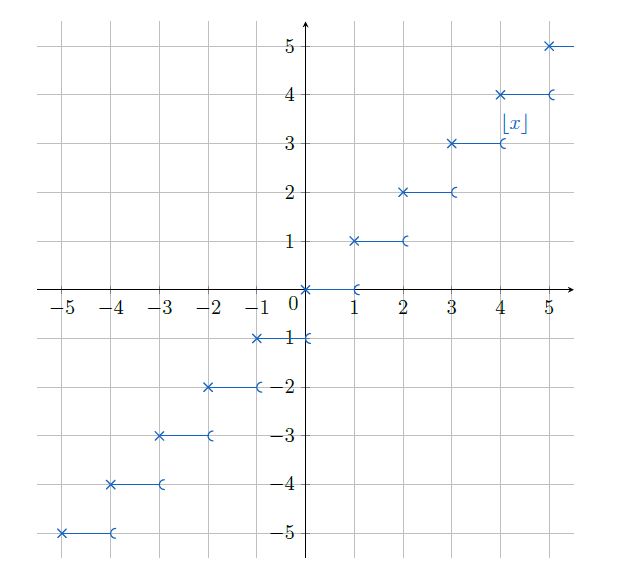
\includegraphics[width=0.7\textwidth]{image2.png}
		\end{figure}
		
\end{document}